\documentclass[bibliography=totoc,listof=totoc,BCOR=5mm,DIV=12,fontsize=12pt,headings=big]{scrbook}

\usepackage[backend=biber, %% Hilfsprogramm "biber" (statt "biblatex" oder "bibtex")
style=ieee, %% Zitierstil (siehe Dokumentation)
natbib=true, %% Bereitstellen von natbib-kompatiblen Zitierkommandos
hyperref=true, %% hyperref-Paket verwenden, um Links zu erstellen
sortcites=true,
sorting=none,
citestyle=numeric-comp
]{biblatex}
\AtEveryBibitem{%
	\clearfield{url}%
     \clearfield{urlyear}
}

% use this declaration to set specific page margins
%\usepackage[a4paper , lmargin = {2.7cm} , rmargin = {2.9cm} , tmargin = {2.7cm} , bmargin = {4.6cm} ]{geometry}
\usepackage{fancyhdr}
\usepackage[a4paper]{geometry}
\usepackage{mathptmx}
\usepackage{amsmath}
\usepackage[english]{babel}
\usepackage{graphicx} 				% it's recommended to use PDF images but you can use JPG or PNG as well
\usepackage{hyperref}
\usepackage{url}           		% format URLs
\usepackage{listings, color}	% for source code
\usepackage{subfig}						% two figures next to each other (example: figure 3a), figure 3b)
% set path where images are stored
\usepackage{csquotes}
\usepackage{scrhack}
\graphicspath{{./img/}}
\addto\extrasenglish{
  \renewcommand{\chapterautorefname}{Chapter}
}
%%
% der Befehl \hypenation versteht keine Sonderzeichen, also weder �
% noch "a noch \"a. W�rter die derartige Zeichen enthalten m�ssen
% direkt im Text getrennt werden, z.B. W�r\-ter
%
\hyphenation{te-le-com-muni-cation 
te-le-com-muni-cation-specific 
Te-le-kom-mu-ni-ka-tions-API} 					% use this file to set explicit hyphenations (doesn't seem to work correctly)
\addbibresource{./bib/references.bib}

\setlength{\parskip}{\baselineskip}
\setlength\parindent{0pt}
\pagestyle{fancy}
\fancyfoot{} % clear all footer fields
\fancyfoot[LE,RO]{\thepage}
\fancyfoot[LO,RE]{Niklas Sprengel}
\fancyhead{}
\fancyhead[LE,RO]{\nouppercase{\rightmark}}
\fancyhead[LO,RE]{\nouppercase{\leftmark}}
\renewcommand{\footrulewidth}{1pt}
\usepackage{acro}
\acsetup{pages/display=all, uppercase/list, barriers/use=true, barriers/reset=true}
\DeclareAcronym{cnn}{
	short = CNN,
	long = convolutional neural network
}
\DeclareAcronym{rgb}{
	short = RGB,
	long = {red, green and blue}
}
\DeclareAcronym{enmap}{
	short = EnMAP,
	long = Environmental Mapping and Analysis Program
}
\DeclareAcronym{gan}{
	short = GAN,
	long = generative adversial network
}
\DeclareAcronym{svm}{
	short = SVM,
	long = support vector machine
}
\DeclareAcronym{ann}{
	short = ANN,
	long = artifical neural network
}
\DeclareAcronym{caf}{
	short = CAF,
	long = cross-layer adaptive fusion
}
\DeclareAcronym{mlp}{
	short = MLP,
	long = multi-layer perceptron
}
\DeclareAcronym{png}{
	short = PNG,
	long = portable network graphics
}
\DeclareAcronym{jpeg}{
	short = JPEG,
	long = JPEG
}
\DeclareAcronym{gpu}{
	short = GPU,
	long = graphical processor unit
}
\DeclareAcronym{vnir}{
	short = VNIR,
	long = visible and near infrared
}
\DeclareAcronym{swir}{
	short = SWIR,
	long = shortwave infrared
}
\DeclareAcronym{asi}{
	short = ASI,
	long = Italian Space Agency
}
\DeclareAcronym{prisma}{
	short = PRISMA,
	long = PRecursore IperSpettrale della Missione
Applicativa,
first-style=short-long
}
\DeclareAcronym{gsd}{
	short = GSD,
	long = ground sampling distance,
}
\DeclareAcronym{s2}{
	short = S2,
	long = Sentinel-2,
}
\DeclareAcronym{esa}{
	short = ESA,
	long = European Space Agency,
}
\DeclareAcronym{btc}{
	short = BTC,
	long = Block Truncation Coding,
}
\DeclareAcronym{heic}{
	short = HEIC,
	long = High Efficiency File Format,
}
\DeclareAcronym{dct}{
	short = DCT,
	long = discrete cosine transform,
}
\DeclareAcronym{dwt}{
	short = DWT,
	long = discrete wavelet transform,
}
\DeclareAcronym{klt}{
	short = KLT,
	long = Karhunen-Loeve transform,
}
\DeclareAcronym{dft}{
	short = DFT,
	long = discrete Fourier transform,
}
\DeclareAcronym{td}{
	short = TD,
	long = Tucker decomposition,
}
\DeclareAcronym{pca}{
	short = PCA,
	long = principal component analysis,
}
\DeclareAcronym{ccsds}{
	short = CCSDS,
	long = Consultative Committee for Space Data Systems,
}
\DeclareAcronym{oned}{
	short = 1D,
	long = one-dimensional,
}
\DeclareAcronym{twod}{
	short = 2D,
	long = two-dimensional,
}
\DeclareAcronym{threed}{
	short = 3D,
	long = three-dimensional,
}
\DeclareAcronym{relu}{
	short = ReLU,
	long = rectified linear unit,
}
\DeclareAcronym{lrelu}{
	short = LeakyReLU,
	long = leaky rectified linear unit,
}
\begin{document}
% ---------------------------------------------------------------
    \thispagestyle{empty}
\begin{center}

{\LARGE \textbf{Technische Universit{\"a}t Berlin}}

\vspace{0.6cm}

{\large Faculty of Electrical Engineering and Computer Science\\[1mm]}
{\large Dept. of Computer Engineering and Microelectronics\\[1mm]}
{\large \textbf{Remote Sensing Image Analysis Group}\\[5mm]}

\vspace*{0.5cm}


\includegraphics[width=5.64cm]{tu_logo_lang_rgb_rot.jpg} % include tu logo

\vspace{0.2cm}
\begin{center}
\rule{0.85\textwidth}{.4pt}
\end{center}
\vspace{0.2cm}
{\LARGE \textbf{Learning-Based Hyperspectral Image Compression Using A Spatio-Spectral Approach}} %TODO change to middle 
\begin{center}
\rule{0.85\textwidth}{.4pt}
\end{center}
\vspace{0.5cm}
{\LARGE Master of Science in Computer Science}\\
\vspace*{0.2cm}
{\large 3 October, 2023}\\ % 	date of submission
\vspace*{0.5cm}
{\LARGE \textbf{Niklas Sprengel}}
\\
\vspace*{0.5cm}
{\large Matriculation Number: 380009} \\
\vspace*{0.5cm}
\begin{flushleft}
\hspace*{1.2cm}
{\large \textbf{Supervisor:}} \hspace*{0.5cm} {\large Prof. Dr. Beg{\"u}m Demir}\\
\vspace*{0.5cm}
\hspace*{1.2cm}
{\large \textbf{Advisor:}} \hspace*{1.15cm} {\large Martin Hermann Paul Fuchs}
\vspace{2cm}
\end{flushleft}

\end{center}




   	\thispagestyle{empty}
    
    \pagenumbering{roman} % use roman number for numbering
    
    \newpage

\thispagestyle{empty}

\begin{large}
\vspace*{1.4cm}
\noindent
\begin{center}
{\Large \textbf{Sworn Affidavit}}
\end{center}

\vspace*{0.5cm}

\noindent
I hereby declare that the thesis submitted is my own, unaided work, completed without any unpermitted external
help. Only the sources and resources listed were used.
\vspace{1cm}

\noindent
Berlin, Date

\vspace{3cm}

\hspace*{7cm}%
\dotfill\\
\hspace*{8.5cm}%
\begin{flushright}
\textit{Niklas Sprengel}
\end{flushright}

\end{large}
 
    \thispagestyle{fancy}
    
    \thispagestyle{empty}
\vspace*{1.4cm}

\begin{center}
    {\Large \textbf{Abstract}}
\end{center}

\vspace*{0.5cm}

\noindent
Learning-based hyperspectral image compression is an increasingly important field of study in the field of remote sensing. This thesis proposes \ac{mymodel}, a novel, highly flexible architecture to perform image compression exploiting both spatial and spectral dependencies of hyperspectral image data. \ac{mymodel} allows for the combination of different spectral and spatial autoencoder models. It further allows spatial autoencoder methods that are optimised for image compression on RGB or multispectral images to be used in the domain of hyperspectral imaging. We propose multiple spectral and spatial models to be used as part of \ac{mymodel} and a training methodology specific to \ac{mymodel} as well as a novel loss function. The models are evaluated on the large-scale hyperspectral image dataset HySpecNet-11k. We analyse the different aspects of the \ac{mymodel} architecture and its training process and compare the achieved reconstruction accuracy for multiple compression ratios. The results show that the \ac{mymodel} architecture significantly improves upon state-of-the-art learning-based hyperspectral image compression methods as well as JPEG 2000 for low and very low bitrates.
\\
    \thispagestyle{fancy}
    \clearpage
    
    \let\cleardoublepage=\clearpage % remove sperate blank page after toc, picture, and etc.
    
    \tableofcontents
    \thispagestyle{fancy}
    
    \printacronyms
    \thispagestyle{fancy}
    
    \listoffigures
    \thispagestyle{fancy}
    
    \listoftables
    \thispagestyle{fancy}
    
    \clearpage
	\pagenumbering{arabic} % use arabic number for numbering
% --------------------------------------------------------------

\mainmatter % comment single chapters for faster compilation

    \chapter{Introduction\label{cha:chapter1}}
Hyperspectral imaging is a quickly growing field. It is the technique of capturing images with a specialized camera to obtain a spectrum of hundreds of wavelengths of light for each pixel of a taken image. Three categories of hyperspectral cameras are used to capture such images. The first, push broom scanners, use a linear arrangement of spectroscopic sensors, that are sensors able to capture a spectrum of many wavelengths of light at once. The sensor arrangement is then moved over the subject of the image, for example by being attached to a satellite orbiting earth. The second category, whisk broom scanners, functions similarly to push broom scanners with the difference being that the stationary sensor arrangement is replaced by a moving mirror reflecting light into a single detector that collects the spectral information in a step-by-step manner. Lastly, snapshot hyperspectral imaging works by using a sensor array to capture a complete hyperspectral image with a single activation of the sensors. 

Regardless of the capture method, there are many applications for the use of hyperspectral images since a multitude of information can be extracted from their combination of spatial and spectral data. One such application is pixel-wise classification of materials, that being the process of determining the material of specific pixels in a hyperspectral image. This is possible because of the high amount of information present per pixel resulting from the large amount of spectral information. An instance of this approach can be seen in Zea et al. \citep{zea_leveraging_2022}. They use the classification of hyperspectral images to detect the presence of the toxic metal cadmium in soil, lessening the need for chemical methods that require the plant to be harvested to test for cadmium stress. Using hyperspectral imaging the detection of cadmium can be performed on living plants. Another example of pixel-wise classification materials is explored in Henriksen et.al. \citep{henriksen_plastic_2022}, where it is used to separate plastic waste by twelve kinds of plastics with a higher accuracy than previously used methods such as near-infrared technology.

Another field where the use of hyperspectral imaging is rising in importance is in geology and environmental sciences. An example of this is the \ac{enmap} mission by \ac{dlr} which launched a satellite into earth orbit in 2022. It takes images of the surface of the earth with a comparatively high \ac{gsd} for hyperspectral sensors of 30 square meters per pixel, allowing for regional geographic analysis \citep{guanter_enmap_2015}. In the spectral domain, the satellite yields a high resolution. By combining a sensor in the \ac{vnir} spectrum and a sensor in the \ac{swir} spectrum it can capture light with wavelengths between 420 and 2450 nm. Wavelengths between 420 and 1000 nm are captured by the \ac{vnir} sensor with a resolution of 6.5 nm per spectral band, while wavelengths between 900 and 2450 nm are captured by the \ac{swir} sensor with a resolution of 10 nm per band.
The \ac{enmap} mission has already led to many interesting studies including glacier ice surface properties of the ice sheet in South-West Greenland, moisture content of soil below grassland and identification of specific crop traits such as the chlorophyll content or the leaf water content \citep{bohn_glacier_2022,pascual-venteo_prototyping_2022,dopper_estimating_2022}.
A dataset created from the images produced by the \ac{enmap} mission also serves as the main dataset studied in this thesis \citep{fuchs_hyspecnet-11k_2023}.

Another ongoing hyperspectral imaging mission is the \ac{prisma} mission led by the \ac{asi} that was launched in 2019 \citep{loizzo_prisma_2019}. Similar to the \ac{enmap} mission, the \ac{prisma} mission also consists of a satellite that observes Earth using both a sensor for the \ac{vnir} spectrum and the \ac{swir} spectrum. It also has a \ac{gsd} of 30 square meters per pixel and a slightly lower spectral resolution given as less than 12 nm per band \citep{guarini_overview_2017,guarini_prisma_2018}. In contrast to the \ac{enmap} mission the satellite also carries a panchromatic camera, meaning that the camera only has a single spectral band. This camera however has a higher \ac{gsd} of 5 square meters per pixel. The data from the \ac{prisma} mission has been used to increase spatial resolution in hyperspectral images. This was done by combining the original hyperspectral images with multispectral images with a higher spatial resolution in a process called hyperspectral-multispectral fusion \citep{acito_prisma_2022}. The term 'multispectral image' refers to images with more spectral bands than traditional \ac{rgb} images, but fewer bands than hyperspectral images. Here the multispectral images contain 10 bands and are obtained from the \ac{s2} project, a mission by the \ac{esa} that continually performs multispectral imaging with fine spatial resolution \citep{drusch_sentinel-2_2012}. Another use of the \ac{prisma} data has been in disaster monitoring where it has been used to segment wildfires into areas of active fire, smoke, burned ground, bare soil and remaining vegetation \citep{spiller_transfer_2022}. Another related system developed using \ac{prisma} data performs wildfire detection in real-time from satellites  \citep{spiller_wildfire_2022}.

The increasing usage of hyperspectral imaging makes it essential to address the disadvantages of the technology. One major disadvantage of this type of imaging is the required amount of disk space for the resulting images. Because there are many more spectral bands compared to the three bands of \ac{rgb} in traditional photography the resulting file size rises accordingly. Furthermore, hyperspectral images often use a high precision for the specific brightness values captured for each point in the image. The \ac{enmap} sensor has a resolution of 14 bits per pixel per band, while in \ac{rgb} imaging 8 bits per pixel per band is the most common \citep{guanter_enmap_2015}. A hyperspectral image might for example have 300 bands. In combination with a higher resolution per pixel per band, the resulting file size would be many times larger than an \ac{rgb} image with the same pixel density. In addition to this, it is important to notice that even \ac{rgb} images need to be compressed for many use cases to be efficiently stored and transmitted, which is why there are many compression standards for \ac{rgb} images in wide usage.
Furthermore, the compression of hyperspectral images is a complex problem. This arises from the combination of spatial image compression complexities and the added challenge of encoding information in the spectral dimension which \ac{rgb} compression algorithms do not consider. The latter is one of the reasons why many \ac{rgb} compression algorithms do not perform well on hyperspectral data as will be shown in this thesis. In addition to this, there are more technical reasons for the difficulty of adapting algorithms for \ac{rgb} compression that will also be explored in this thesis. For the above-mentioned reasons, research into compression algorithms for hyperspectral images is of vital importance.

Algorithms for image compression can be categorized into multiple broad groups. They can firstly be grouped by whether they compress the image losslessly or with loss. Lossless algorithms restore the compressed image exactly, whereas lossy reconstructions cause distortion. The disadvantage of lossless compression is however that there are mathematical limits to the compression rate given by the entropy in the data that is to be compressed. This limit is given by Shannon's source coding theorem \citep{shannon_mathematical_1948}, which has been stated as follows \citep{mackay_information_2003}:

\begin{quotation}
$N$ independent identically distributed random variables each with entropy $H(X)$ can be compressed into more than $N\cdot H(X)$ bits with negligible risk of information loss, as $N \rightarrow \infty$; but conversely, if they are compressed into fewer than $NH(X)$ bits it is virtually certain that information will be lost.
\end{quotation}

This means that the average bitrate, the compression rate given by the quotient of input bits and output bits of the compression algorithm, which is achievable using lossless compression algorithms is given by the entropy of the data that is to be compressed.
In contrast, lossy compression methods can achieve much higher compression rates by allowing the introduction of distortion. Furthermore, they can also adapt their rate of compression based on either the desired amount of distortion or the target compression rate. They can also be combined with a lossless compression method to further optimise their compression rate. 
Another important factor that determines the trade-off between lossless and lossy compression methods is that many applications do not require the perfect reconstruction given by lossless methods. For example, García-Vílchez et al. \citep{garcia-vilchez_impact_2011} showed that in hyperspectral image classification, lossy compression of the image does not always reduce the performance of the classifier. For some lossy compression algorithms, the classifier even produced better results on the compressed data than the uncompressed data. This is explained by an introduction of smoothing from the compression which is advantageous for the \ac{svm} classifier used in the experiment. 
For these reasons, this thesis focuses on lossy compression methods.

Lossy compression algorithms can be further categorized into traditional compression methods and learning-based compression methods. Traditional compression methods employ algorithms such as the discrete cosine transform which is used in the \ac{jpeg} image compression standard or the wavelet transform, often in combination with a lossless entropy coding method. Examples of traditional methods other than \ac{jpeg} are \ac{btc} which splits images into blocks and then rounds pixel values inside the blocks efficiently and the \ac{heic} standard, which uses wavelet transforms similar to \ac{jpeg} \citep{delp_image_1979,hannuksela_high_2015}. Learning-based approaches use the powerful capability of artificial neural networks to universally approximate arbitrary functions using gradient descent \citep{ruder_overview_2017}. These networks are then used to build models that learn to compress and decompress images. Lately, these networks have been shown to outperform traditional compression methods for many applications, especially for \ac{rgb} images using, for example, the hyperprior model given by Ballé et al.\citep{balle_end--end_2017,balle_variational_2018,minnen_joint_2018} which will be discussed in detail in \autoref{sec:ch2hyperspectral}. 
Research into compression for hyperspectral images is in its early stages, however, even in this domain, promising results are showing the capabilities of learning-based autoencoders for this task \citep{kuester_1d-convolutional_2021,kuester_transferability_2022,la_grassa_hyperspectral_2022,guo_learned_2021}.

\section{Objective\label{sec:objective}}
This thesis addresses the problem of hyperspectral image compression using deep learning models consisting of two parts, an encoder and a decoder.
The encoder learns to map the original image to a low-dimensional latent space, thereby performing compression. Analogously, the decoder is trained to reconstruct the input by mapping elements from this latent dimension to full-size images that are as close as possible to the original image.

Contributions to the research on learning-based hyperspectral image compression are made in this thesis by introducing a new architecture that enables the use of spatial compression algorithms such as models that might be used for \ac{rgb} image compression by combining them with a model that performs compression in the spectral domain while keeping spatial relationships intact. In this way, it is possible to compress the spatial information in hyperspectral images using models that are not ordinarily applicable to such images.

Using this architecture, multiple model combinations are designed and compared with each other as well as with the base versions of these models.
These models include models based on \acp{cnn} as well as transformer-based architectures.
A model using a hyperprior architecture is also used for spatial compression. This architecture yields much higher compression ratios than other models by using an arithmetic encoder in the bottleneck of the compression model. In this way, compression rates much higher than the current state of the art for hyperspectral image compression are achieved while distortion is only reduced by a comparatively small amount. 

Additionally, the latent spaces of both the encoder in the spectral domain as well as the latent space of the spatial encoder will be analysed.

\section{Outline\label{sec:outline}}
This section gives a brief introduction of the 7 chapters into which this thesis is split.

\textbf{\autoref{cha:chapter2}} presents the related work. This relates to the research of learning-based hyperspectral image compression by itself. However, as learning-based compression for hyperspectral images, in contrast to traditional hyperspectral compression methods, is a recent and relatively unexplored field of study, the adjacent research topic of learning-based \ac{rgb} image compression is also explored. There is also some exploration of the general studies done on convolutional neural networks as well as transformers.

\textbf{\autoref{cha:chapter3}} gives an overview of the theoretical ideas used in the proposed methods, such as \acp{cnn}, transformers, arithmetic coding as well as the hyperprior architecture for compression.

\textbf{\autoref{cha:chapter4}} details the individual submodels making up the models that are proposed to address the hyperspectral image compression problem as well as the models in their totality. It also gives an overview of the loss functions used for training the models, one of which is a loss function specifically designed for the models proposed in this thesis.

\textbf{\autoref{cha:chapter5}} explains the design of the performed experiments, the dataset that is used for these experiments as well and the results of these experiments. It also details some of the challenges encountered during the experimentation phase.

\textbf{\autoref{cha:chapter6}} gives a summary of the results from the thesis as well as possible improvements that could be made as well as ideas that could be explored in future research.

    \thispagestyle{fancy}
    \acbarrier
    \chapter{Related Work\label{cha:chapter2}}
\section{Hyperspectral image compression \label{sec:ch2yyy}}
\subsection{CNN-based architectures}
\subsection{Transformer-based architectures}
\section{RGB image compression \label{sec:ch2xxx}}
\subsection{CNN-based architectures}
\subsection{Transformer-based architectures}
\section{ZZZ \label{sec:ch2zzz}}
    \thispagestyle{fancy}
    \acbarrier    
    \chapter{Theoretical Foundations\label{cha:chapter3}}
This thesis employs multiple different types of machine learning and compression methods, such as \acp{cnn}, self-attention modules, arithmetic coders and the hyperprior architecture. The following sections briefly explain foundations in these topics in order to aid the understanding of the models proposed in this thesis.
\section{Convolutional Neural Networks}
\begin{figure}[t]
\centering
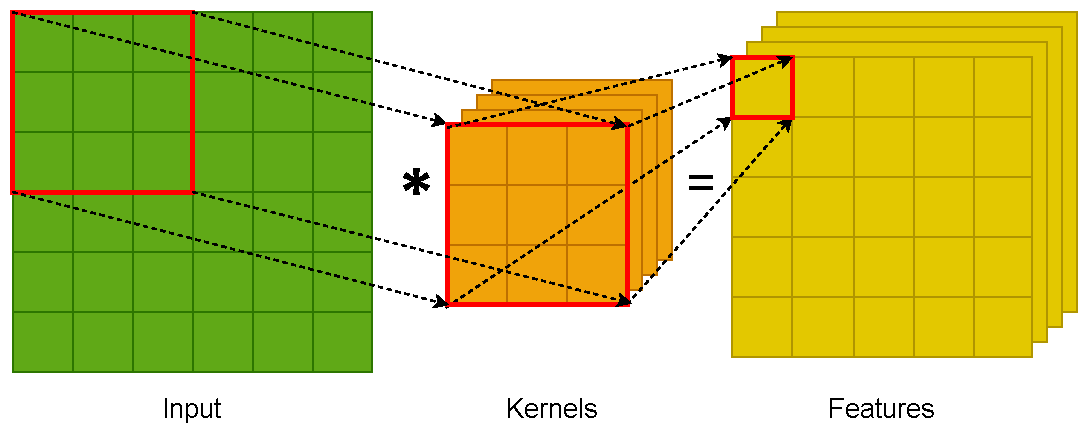
\includegraphics[scale=0.8]{CNN.pdf}
\caption[Example of convolutional layer]{Example of a \ac{twod} convolutional layer computing a feature pixel.}
\label{fig:cnn}
\end{figure}

\Acp{cnn} are a type of \ac{ann}, distinguished from other \acp{ann} by the fact that they use convolutional layers as part of their architecture \citep{oshea_introduction_2015}. They were originally designed for the purpose of image classification, which remains one of the main applications for \acp{cnn} \citep{gu_recent_2018}. However, \acp{cnn} are also used in other fields of machine learning such as \ac{nlp}. The most common type of \ac{cnn} in the field of computer vision uses \ac{twod} convolutional layers in combination with subsampling or pooling layers and activation functions in order to learn features of an input image. 

A \ac{twod} convolutional layer takes a \ac{twod} image-like input and produces a given number of features each represented as a \ac{twod} matrix \citep{gu_recent_2018}. These features are computed for a given pixel by convolving the neighbourhood of this pixel with a kernel, which is shown in \autoref{fig:cnn}. These kernels are comprised of the weights of the convolutional layer and are therefore learned using gradient descent. A pooling layer is then used to reduce the spatial dimensionality of the input. Such a combination of a convolutional and a pooling layer can be repeated multiple times, since the output of both the convolutional layer and most pooling layers are again image-like and can be used as input to additional such layers. Between sets of convolutional and pooling layers nonlinear activation functions are applied in order for the network to be able to learn nonlinear features. The combination of multiple sets of convolutional and pooling layers  is central to learning-based image compression and is used in a multitude of the proposed models \citep{balle_end--end_2017,balle_variational_2018,kuester_1d-convolutional_2021,kuester_transferability_2022,guo_learned_2021}.

Compared to other neural network architectures such as \acp{mlp}, \acp{cnn} have low complexity because of the small number of connections between neurons, as each output neuron of a convolutional layer is only connected to a small number of neurons from the input of the convolutional layer, defined by the kernel size \citep{gu_recent_2018}. The low complexity results in \acp{cnn} being resilient to overfitting \citep{oshea_introduction_2015,gu_recent_2018}. However, regardless of the low complexity, \acp{cnn} are still able to learn high-level features of the input because the use of multiple convolutional layers allows for a hierarchical learning of features. This allows the early convolutional layers to learn to detect low-level features such as corners or edges while the later convolutional layers learn higher-level features \citep{gu_recent_2018}

In addition to the \ac{twod} convolutional layer, there are other variations of convolutional layers that are useful, in particular for analysing hyperspectral image data. Firstly, one can define a \ac{oned} convolutional layer, which differs from the \ac{twod} layer in that the kernel moves only in a single dimension. In hyperspectral image analysis this can be used to learn spectral information, since this information is \ac{oned} \citep{kuester_1d-convolutional_2021,kuester_transferability_2022}. Similarly, \ac{threed} convolutional layers can be defined by using a \ac{threed} cube-shaped kernel. In hyperspectral image processing, this type of layer can be used to learn features of the spatial and spectral domain within a single layer \citep{guo_learned_2021}.

\section{Self-Attention modules}
The self-attention mechanism is a technique that is widely used in the field of \ac{nlp}. For example, Vaswani et.al. \citep{vaswani_attention_2017} used it as the main part of their proposed transformer architecture which outperformed other machine-learning approaches in various \ac{nlp} tasks at the time, such as language translation. The mechanism aims to compute a latent representation of an input sequence by learning to relate the elements of the input sequence to each other. While a \ac{cnn} can also achieve this, in a \ac{cnn} only elements close to one another are used to compute the latent representation. Using self-attention, the relation of all elements with all other elements can be incorporated, enabling learning of long-distance dependencies \citep{vaswani_attention_2017}.

In recent years, self-attention modules have also been used in computer vision. In image compression for example, self-attention modules can be used in order to enable the neural network focus on the more complex parts of the input image and subsequently use less bits for the compression of the less complex parts of the input, improving the overall compression\citep{cheng_learned_2020, liu_non-local_2019}. 

\section{Arithmetic Coding}
\label{sec:arithmetic}
Arithmetic coding is an algorithm used for entropy coding, that being a technique for encoding and decoding a sequence of symbols in an efficient way \citep{witten_arithmetic_1987}. As an example, a string of characters can be considered. A standard non-optimized method of storing a string is by using the \ac{ascii} encoding which used a fixed seven bytes per character of the string. Entropy coding algorithms improve on this by allocating fewer bits to more common characters and therefore more bits to less common characters \citep{witten_arithmetic_1987}. In total, this leads to a lower number of required bits for the total message, given an accurate probability model for the frequencies of the characters. In fact, if the provided probability model is perfectly accurate, arithmetic coding yields an encoding close to an optimal encoding, that being an encoding that uses a number of bits equal to the entropy of the encoded input \citep{witten_arithmetic_1987}. This is the fewest number of bits possible for a lossless encoding of an arbitrary message, which was proven with Shannon's source coding theorem \citep{shannon_mathematical_1948,mackay_information_2003}.

\begin{figure}
\centering
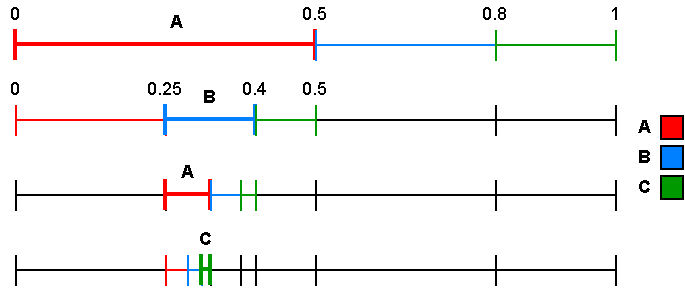
\includegraphics[scale=1]{ArithmeticCoding.pdf}
\caption{Arithmetic coding process of the character sequence "ABAC".}
\label{fig:arithmetic}
\end{figure}

Arithmetic coding, using the theoretical version of the algorithm, works by encoding the entire input message into one arbitrary-precision rational number $q$ with $0 \leq q < 1$ \citep{said_introduction_2023}. In practice the algorithm is slightly modified to account for the lack of infinite precision in computers, as will be detailed later in this section. The encoding is performed using an iterative process. In order to understand this process, consider for an example an alphabet consisting of three symbols, 'A', 'B' and 'C' with 'A' having the probability $0.5$, 'B' having the probability $0.3$ and therefore 'C' having the probability $0.2$. Encoding a message is performed symbol by symbol. To encode the first symbol, the interval $[0,1)$ (meaning numbers $a$ with $0 \leq a < 1$) is split into three parts according to these probabilities. If the first symbol is 'A', the final encoding number $q$ will be in the interval $[0,0.5)$. Likewise, if the first symbol is 'B' or 'C', $q$ will be in the intervals $[0.5,0.8)$ or $[0.8,1)$ respectively. The second symbol is then encoded by splitting the interval determined from the first symbol again, using the same probabilities. A sequence of two 'A' symbols would therefore result in $q$ being in the interval $[0,0.25)$. This procedure is iterated until each symbol of the input message is encoded, resulting in a single number $q$ representing the entire input. This process can be seen in \autoref{fig:arithmetic} using the aforementioned probabilities for the word "ABAC". This number encodes the original message nearly optimally given a perfect probability distribution, with a difference of less than a bit to the entropy of the message. The reason for this discrepance is that $q$ is always represented using an integer amount of bits. If the input image has a non-integer entropy, the required amount of bits to store $q$ is the entropy rounded up to the nearest integer. However, the complete algorithm of arithmetic encoding requires an additional source of information that needs to be transmitted to the decoder. In order to decode the message, the decoder needs to know the probability model as well as a way to distinguish when the message ends. The first is constant with respect to message length. The second can be transferred using only logarithmic overhead with respect to message length. This is often done by adding an additional token that signifies the end of the message \citep{said_introduction_2023}.

As mentioned before, the algorithm is adapted slightly in practice in order to use fixed precision numbers instead of arbitrary precision numbers. Rounding operations as a result of using fixed point numbers are the same for encoder and decoder and therefore do not inhibit the algorithm in principle. However, as a result of rounding, intervals can become small enough that they are not representable with fixed point numbers of the used precision. In this case, the intervals are changed in a determinable way so that they are again representable. This process is called renormalization and multiple algorithms to perform this procedure exist.
Arithmetic coding also allows for the possibility of changing the probability distribution during the encoding process based on previously encoded symbols. This is possible because the decoder decodes the symbols in the same order as the encoder encodes them and can therefore perform the same change to the probability distribution as the encoder, as long as the method for changing the probability model was decided beforehand \citep{said_introduction_2023}. An example of such an algorithm is \ac{cabac}, which is an entropy coding method used in the video encoding standards \ac{avc} and \ac{hevc} as well as multiple learning-based \ac{rgb} compression models \citep{balle_end--end_2017,balle_variational_2018,minnen_joint_2018}. \Ac{cabac} is a binary encoding method, therefore requiring the data that is to be encoded to be transformed beforehand. It works by using multiple probability models and, for each element that is to be encoded, selecting one of these models based on previously encoded elements \citep{sze_high_2012}. Since the choice of probability model for each element is only based on elements that were encoded before it, decoding is still possible by performing the same probability model choices as the encoder. Further more, the probability models are updated after each encoding step to adapt them to the data.

In learning-based lossy image compression, arithmetic coding is used as part of the Hyperprior architecture order to encode the latent representation of an input image \citep{balle_end--end_2017,minnen_joint_2018,balle_variational_2018}. The latent representation of the input image and the probability distribution used for the arithmetic coder can be learned using \acp{ann}.

\section{Hyperprior Architecture\label{sec3:hyperprior}}
The hyperprior architecture was first proposed by Ballé et.al. \citep{balle_variational_2018} to improve on an earlier work by Ballé et.al. \citep{balle_end--end_2017}, both in the field of grayscale and \ac{rgb} image compression. In the earlier work, a \ac{cnn} using \ac{twod} convolutional layers, downsampling layers and \ac{gdn} as the activation function was used to transform an input image into a latent representation. This network is called the analysis transform. The latent representation is then compressed using an arithmetic coder. Afterwards, another \ac{cnn} is used to transform the decoded output from the arithmetic coder. This \ac{cnn}, called the synthesis transform, is symmetric to the analysis transform in that it contains the same convolutional layers in inverse order. Additionally, instead of downsampling layers and \ac{gdn} upsampling layers and the activation function \ac{igdn} is used. The whole model is then trained using a loss function called rate-distortion loss that optimizes for compression rate and reconstruction distortion simultaneously. Since the arithmetic coder performs lossless compression and the compression rate of the \ac{cnn} is fixed, optimizing the compression rate corresponds to optimizing the probability distribution estimate of the arithmetic coder and optimizing the distortion corresponds to optimizing the quality of the reconstruction produced by the \acp{cnn}. A disadvantage of this approach is that the probability distribution used for the arithmetic coder is a fully factorized distribution, which is not optimal if the latent representation computed by the analysis transform contains statistical dependencies \citep{balle_variational_2018}.

\begin{figure}
\centering
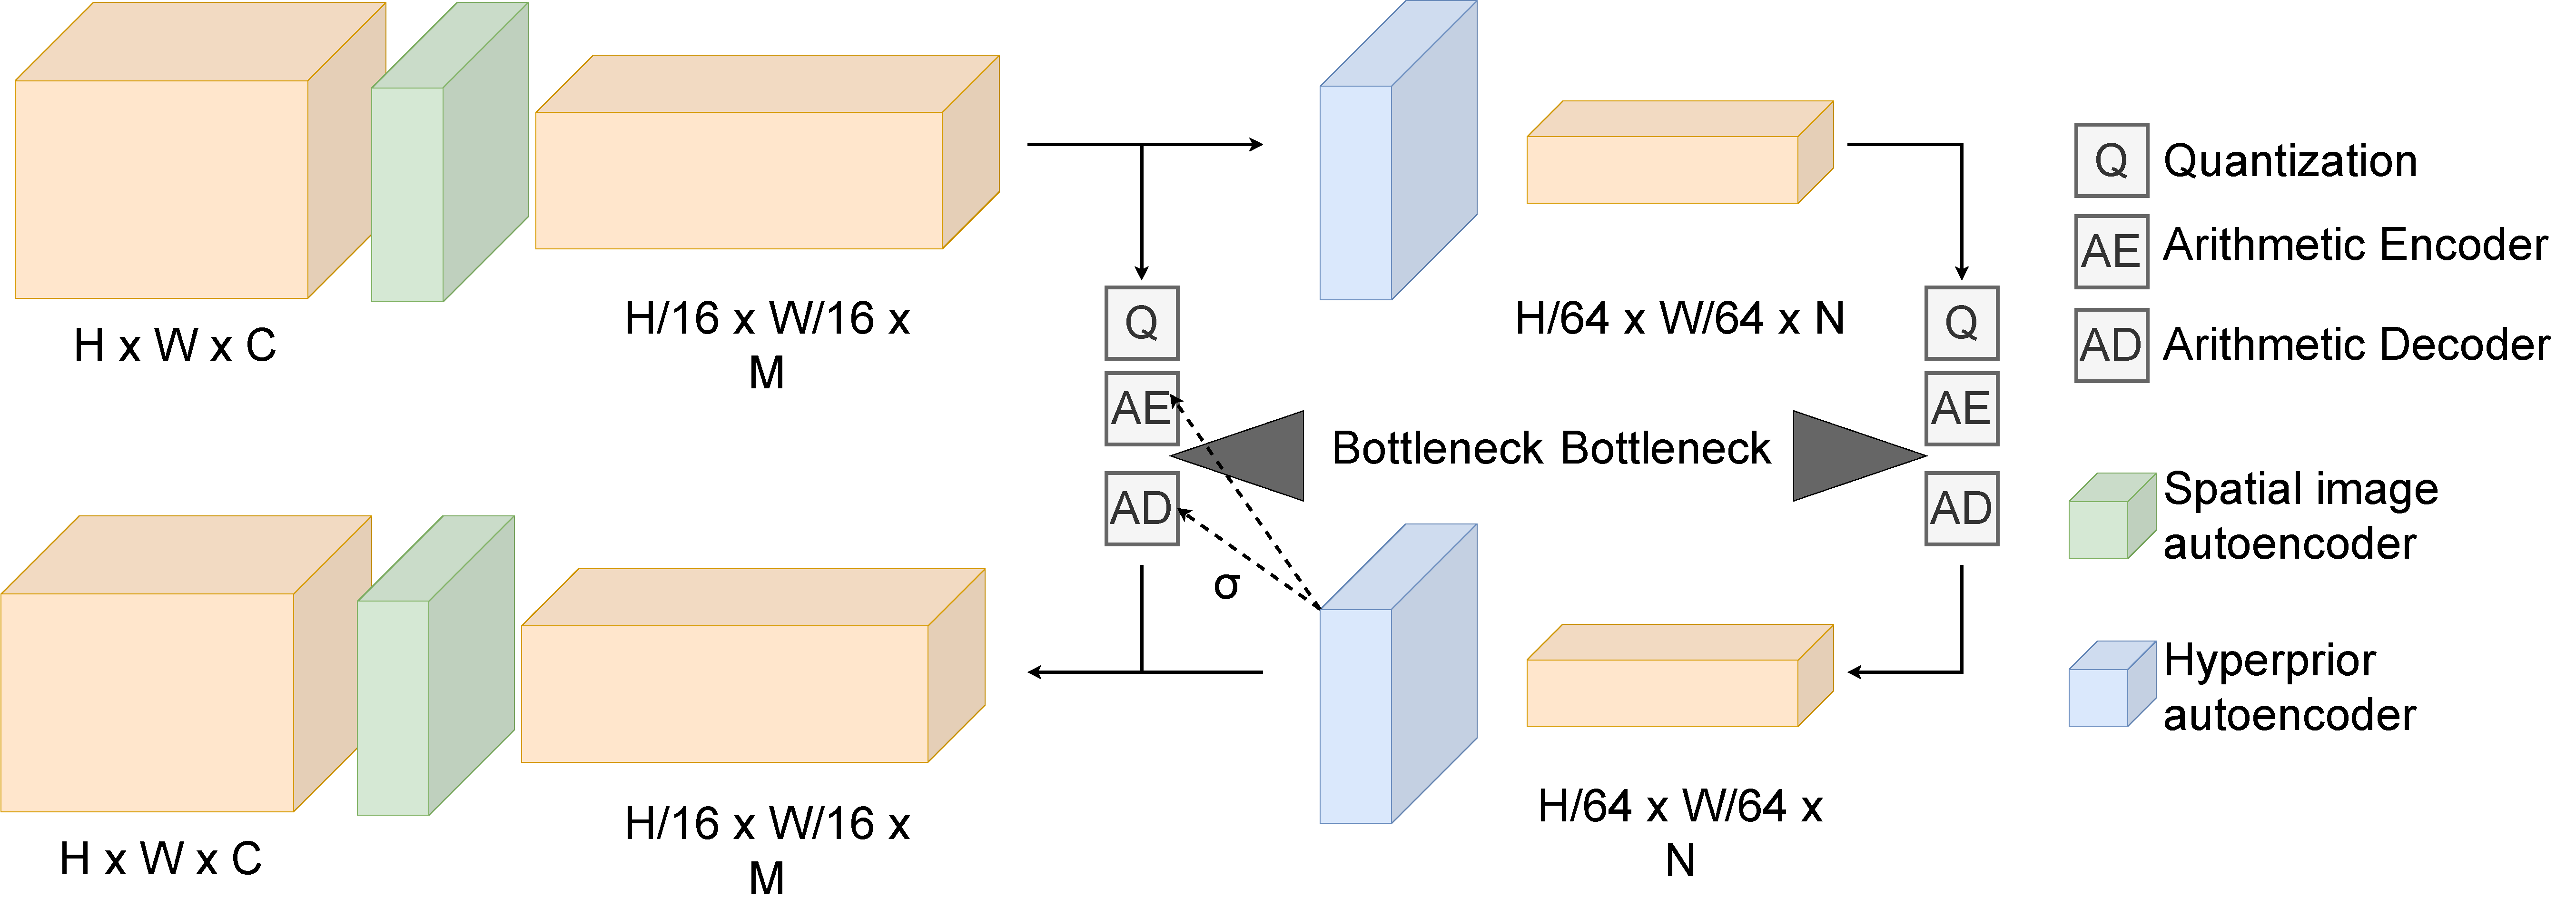
\includegraphics[scale=0.16]{Hyperprior.pdf}
\caption[Scale hyperprior architecture]{Architecture of the variational scale hyperprior model proposed in \citep{balle_variational_2018}.}
\label{fig:hyperprior}
\end{figure}

The hyperprior architecture attempts to solve this problem by transmitting information about the probability distribution of the image that is being compressed as side channel information \citep{balle_variational_2018}. This is in contrast to the former model, in which only the probability distribution of the training dataset as a whole is known to both encoder and decoder. The authors noticed that when modelling the probability distribution with gaussians, the standard deviations of latent pixels near each other in specific images tend to vary from the overall probability distribution in a similar manner. Note that while the latent vectors are not images, they can be interpreted as images by treating the filters as different channels of an image with multiple channels. In this way it is also possible to refer to pixels of latents, referring then to the values of all filters for a specific point in the spatial dimensions. To address the spatial dependencies of the standard deviations of the latents, an additional \ac{cnn} was added to exploit the spatial dependencies in the latents \citep{balle_variational_2018}. This network is called "hyperprior". The hyperprior network is also split into an analysis and a synthesis transform and is therefore similar to a smaller version of the original \ac{cnn}. A visualisation of this architecture is shown in \autoref{fig:hyperprior}. A difference between the networks is that the hyperprior network uses \ac{lrelu} as the activation function instead of \ac{gdn}. This makes sense because \ac{gdn} is shown to be especially useful for improving visual similarity in an image compression network. This is not useful for the hyperprior network since it does not attempt to learn image reconstruction. Instead, the hyperprior network is used to learn the probability distribution of the latents of the main \ac{cnn}. More specifically, the hyperprior analysis transform produces a bottleneck tensor, which can be compressed with an arithmetic coder using a fully factorized distribution similar to the earlier work by Ballé et.al. \citep{balle_end--end_2017}. The hyperprior synthesis transform then predicts the standard deviations for each pixel in the latent of the hyperprior from that bottleneck. This improves the performance of the arithmetic coder significantly, because the probability distribution predicted by the hyperprior network is closer to the true distribution than the fully factorised distribution that was used in the model without a hyperprior network. This is especially true if the analysed dataset is heterogeneous, since the fully factorised distribution by definition is the same for each compressed image, while the inclusion of a hyperprior enables the arithmetic coder to use different standard deviations for the distributions of each image that depend on that specific image \citep{balle_variational_2018}. A tradeoff exists in that in contrast to the non-hyperprior approach, the bottleneck of the hyperprior \ac{cnn} has to be transmitted alongside the image data. However, Ballé et.al. \citep{balle_variational_2018} showed that the advantage of increasing the performance of the main arithmetic coder outweighs the additional bits of information that have to be transmitted.

\begin{figure}
\centering
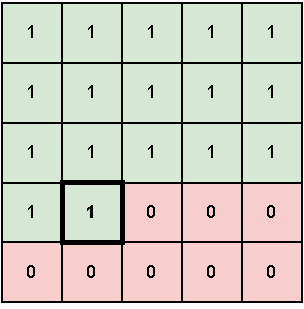
\includegraphics[scale=1]{MaskedConv.pdf}
\caption[Example of masked convolutional layer]{Example of a kernel for a \ac{twod} masked convolutional layer. The pixels to the bottom and right of the current pixel are not used. The current pixel is marked bold.}
\label{fig:maskedconv}
\end{figure}

A further improvement to the hyperprior model was proposed by Minnen et.al. \citep{minnen_joint_2018}, seen in \autoref{fig:hyperpriorcm}. They firstly added a context model to the main arithmetic encoder. This context model adjusts the probability distributions for a specific image during the decoding process based on the already decoded elements. This is a common approach in arithmetic coding \citep{said_introduction_2023}. See also \autoref{sec:arithmetic} for more elaboration on this idea. While the arithmetic coder in the previous models was based on the \ac{cabac} algorithm and therefore also context-sensitive, the context model did not improve the model significantly because images that were to be compressed were fed into the autoencoder sequentially pixel by pixel, which is not optimal \citep{balle_end--end_2017}. Minnen et.al. improves the context model by introducing a masked \ac{twod} convolutional layer applied to to the quantized latents of the main \ac{cnn}. A masked convolutional layer in this case refers to a convoltional layer in which the kernel only contains pixels up and to the left of the currently transformed pixel. This idea, first proposed in Oord et.al. \citep{oord_conditional_2016}, ensures the layer only uses the parts of the input that are at this point known to both the arithmetic encoder and decoder. If a standard convolutional layer would be used, the output of the arithmetic coder would not be decodeable, since it would be partly based on pixels that are not yet decoded.  The output of this layer is then combined with the output of the hyperprior synthesis transform using a three-layer \ac{cnn} with 1x1 kernels to produce the parameters used for the arithmetic coder. Since the inputs to the context model can also be seen as coming from the output of the arithmetic decoder because of the losslessness of the arithmetic coder, the context model can be seen as an autoregressive component improving the probability distribution estimates of the arithmetic coder \citep{minnen_joint_2018}. The other improvement proposed in Minnen et.al. \citep{minnen_joint_2018} is a change from a gaussian scale hyperprior to a \ac{gmm}. In contrast to the hyperprior in Ballé et.al. \citep{balle_variational_2018} that predicted only the standard deviations of the gaussians, the proposed model also predicts the means of the gaussians. This is achieved in the model architecture by making the number of filters in the last layer of the hyperprior synthesis transform and the number of filters in the masked convolutional layer of the context model double the number of filters in the output layer of the main decoder. In this way, for each element in the latent two values in the probability distribution are predicted, the mean and the standard deviation \citep{minnen_joint_2018}.

\begin{figure}
\centering
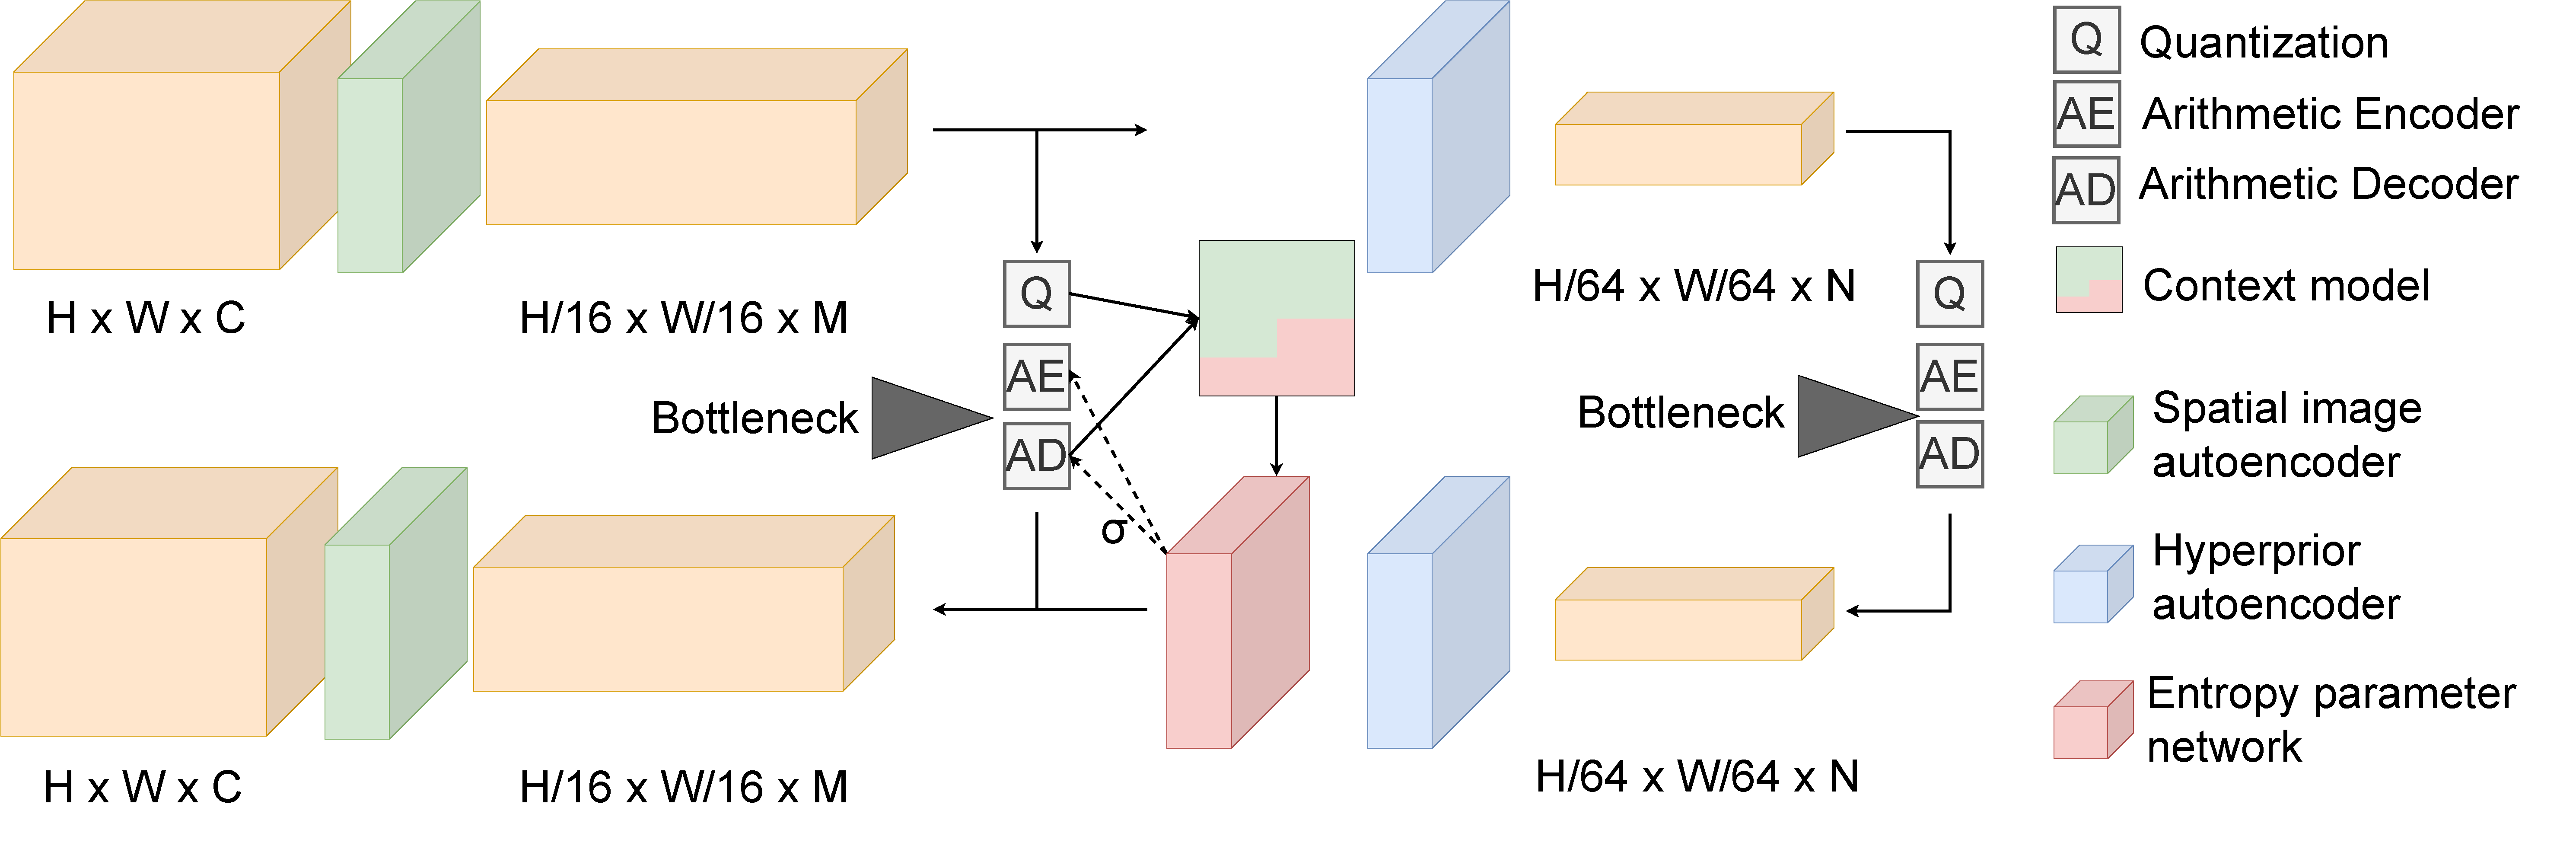
\includegraphics[scale=0.16]{Hyperprior_CM.pdf}
\caption[Joint hyperprior architecture]{Hyperprior model using an autoregressive context model proposed in \citep{minnen_joint_2018}.}
\label{fig:hyperpriorcm}
\end{figure}
    \thispagestyle{fancy}
    \acbarrier    
    \chapter{Methodology\label{cha:chapter4}}
As discussed in \autoref{cha:chapter2}, learning-based compression of \ac{rgb} imagery is a hot topic. Therefore, being able to use and further research methods used in that field for hyperspectral image compression would be useful. However, direct application of most learning-based \ac{rgb} image compression methods on hyperspectral data is not possible. This is mainly for two reasons. Firstly, learning-based \ac{rgb} image compression methods ignore dependencies between the three channels in the \ac{rgb} images and focus solely on spatial dependencies. This is useful for \ac{rgb} images because the spectral dependencies within the three channels are low, since the corresponding wavelengths are far apart. Additionally, having only three channels means that there is not much spectral information per pixel to be compressed, meaning that even if spectral dependencies existed, the compression gains that could be extracted would be small. This is different in hyperspectral image compression where there are large amounts of spectral dependencies and the potential compression gains are much larger because of the high number of spectral channels. It is therefore necessary to modify \ac{rgb} models to incorporate spectral dependencies in order to adapt them to the task of hyperspectral image compression. 

The second reason for the difficulty in applying \ac{rgb} image compression methods to hyperspectral image is the strong increase in spectral dimension. Compared to an \ac{rgb} image, a hyperspectral image of the same size with 200 channels has $200/3 \approx 67$ times more dimensions. For this reason \ac{rgb} models are often too small to learn the compression of high-dimensional hyperspectral image data. For example, many \ac{cnn} models use an input layer transforming the input from the dimensions $H \times W \times C$, where $H$ and $W$ are the height and width and $C$ is the number of channels to $H' \times W' \times N$, where $H'$ and $W'$ are often either the original height and width or half the original height and width and $N$ is the number of filters used in the input layer. If $H'$ and $W'$ are equal to half the original height and width, this is achieved either using a pooling layer or a convolutional layer with a stride of two. In \ac{rgb} models, 128 and 192 are common values for $N$. For \ac{rgb} images, this means that the input layer increases the dimensionality drastically in order to learn multiple features of the image. However, in hyperspectral images, the same layer would result in a decrease of dimensionality leading to loss of information. A simple idea in order to address this issue is to increase the number of filters in each layer according to the increase in dimensionality between \ac{rgb} and hyperspectral images. The input layer would then for example have $192 * 67 = 12864$ filters. However, this idea would result in a much larger model than the corresponding \ac{rgb} compression model and therefore require a higher amount of computational resources for training, potentially making the model impossible to train on the available hardware. Additionally, even if the models were trainable, it is unclear if the convolutional layer would be able to learn 12864 distinct features for hyperspectral images.

Therefore, a different model architecture is needed. This thesis presents a novel architecture that allows the use of spatial compression methods designed for an almost arbitrary number of channels in hyperspectral image compression while also incorporating spectral dependencies. This not only allows the use of \ac{rgb} image compression methods but also multispectral compression methods. This architecture is called "Combined Model" and is shown in \autoref{fig:combined}.
%Furthermore, it is also possible to use non-learning-based methods using a desired number %of channels, like \ac{jpeg} 2000, on hyperspectral data while integrating spectral %dependencies of hyperspectral images. 
\section{The Combined Model\label{sec:combinedmodel}}
\begin{figure}
\centering
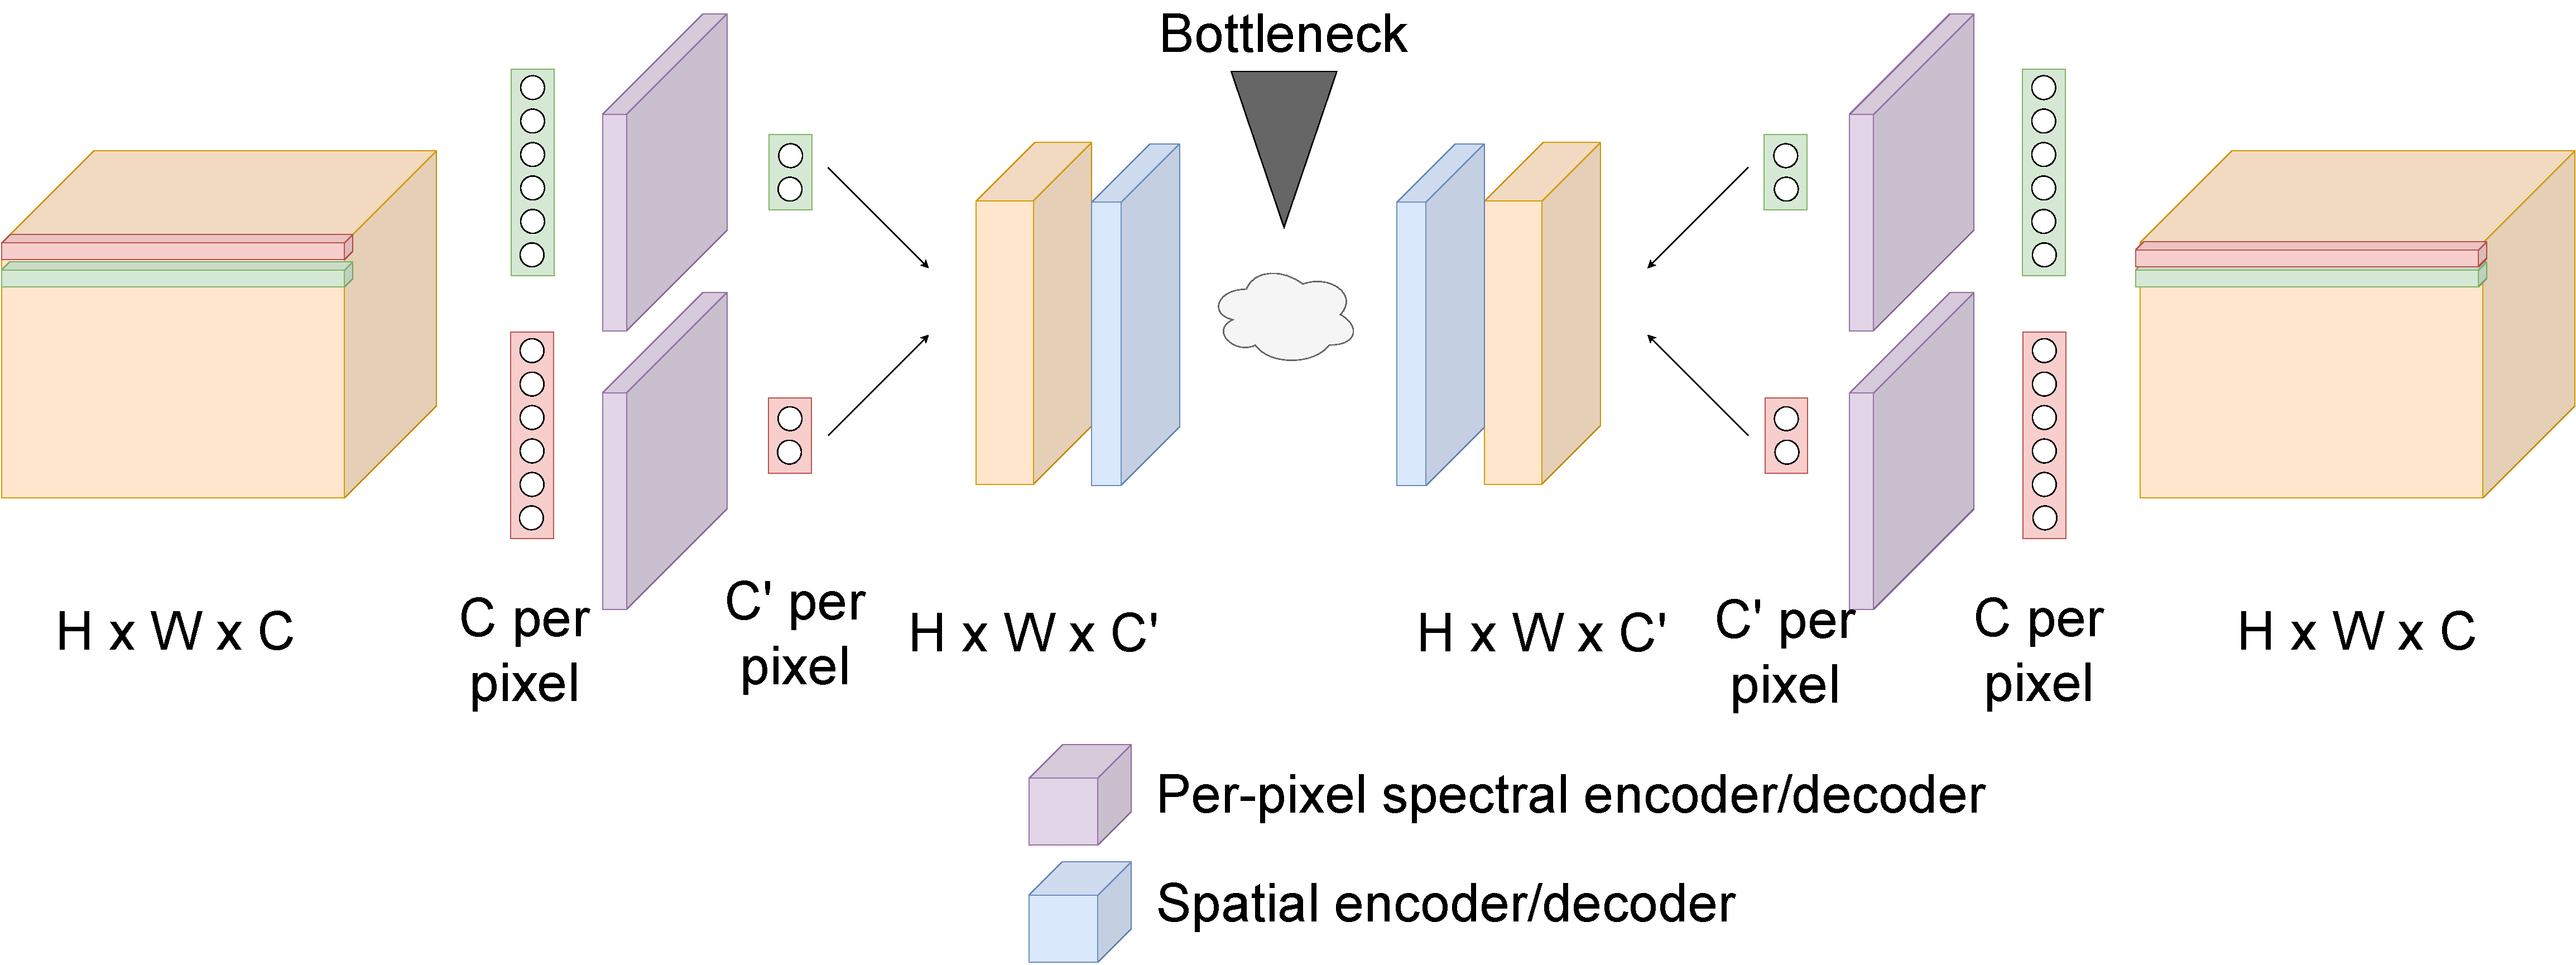
\includegraphics[scale=0.18]{img/GeneralArchitecture.pdf}
\caption[Combined model architecture]{Architecture of the Combined Model using the per-pixel spectral \ac{cnn}}
\label{fig:combined}
\end{figure}

The main idea of the combined model is to use a spectral encoder network that preserves spatial dependencies in order to reduce the number of spectral channels in the input. Then, a spatial compression method is applied on the output of that spectral encoder in order to exploit the spatial dependencies. The resulting bottleneck is then decoded using the corresponding spatial decoder. Finally, a spectral decoder network symmetrical to the spectral encoder restores the original image. During training, the spectral decoder learns to adapt to the distortion introduced by the spatial autoencoder. If the spatial autoencoder is learning-based, the spatial autoencoder similarly learns to produce output in such a way that the spectral autoencoder can better decode it. This mechanism is studied in detail in \autoref{cha:chapter5}. Adaptation in either the spatial autoencoder or the spectral autoencoder are necessary, especially if the latent space of the spectral autoencoder is not continuous. In that case, a small change introduced by the spatial autoencoder could result in a large change in the output of the spectral decoder. In practice the adaptation process is successful in avoiding chaotic outputs of the spectral decoder, which is also shown in \autoref{cha:chapter5}.

The aforementioned approach has multiple advantages. It is highly flexible with regard to the spatial autoencoder. Many different learning-based approaches can be used and the number of input channels to the spatial autoencoder can be modified so it best fits the spatial autoencoder. This can be achieved by modifying the compression ratio of the spectral encoder/decoder pair, which is possible for all spectral autoencoder models studied in this thesis. Another advantage is that the distinct separation between the spatial and the spectral encoding allows for informative studies to be done both regarding explainability and regarding the amount of spatial and spectral dependencies in the data. The model also allows for different spectral encoder and decoder architectures. There are two necessary conditions required for a spectral encoder/decoder pair to be possible for use in the combined model. Firstly, the output of the encoder must be an image-like shape in order for spatial image compression models to be used for incorporating the spatial dependencies. Secondly, the spectral encoder needs to preserve spatial dependencies, ideally resulting in an output with similar spatial dependencies to the actual input image. Because the spatial autoencoder models were designed for image compression, having spatial dependencies close to the dependencies found in images means that the task the spatial autoencoder is used for is close to the one it was designed for.

However, a difference between the task of image compression and the task the spatial autoencoder performs, that being compression of the latent of the spectral autoencoder, is still present. This is one of the disadvantages of the combined model approach and therefore requires the spatial autoencoder to be resilient to this change of task. However, for the spectral autoencoder models studied in this thesis, the spatial dependencies of the latents very closely resemble the spatial dependencies of the original input, mitigating this disadvantage. For further detail on this see \autoref{cha:chapter5}.

For training the combined model, an additional idea is useful. If the model is trained in a standard way by endtraining both the spatial autoencoder and the spectral encoder/decoder pair end-to-end from a newly initialized state at the same time, the results can be unstable. Depending on the hyperparameters, it may not be possible to train the combined model in this way. This follows from the fact that inputs to the spatial autoencoder depend on the outputs of the spectral encoder. During the start of training, the spectral encoder often outputs similar or equal values for all inputs. The spatial autoencoder may then specifically learn to compress latents with these specific values, which is a task very different from compressing spatial dependencies. In this case, the dependencies between the model parts can inhibit training and lead to the model being stuck in the local minimum of outputting the same output for any input. We solve this problem by pretraining the spectral encoder/decoder pair as an autoencoder without any spatial component. Then the combined model is trained using the pretrained spectral encoder and decoder. In this way, the spatial autoencoder receives useful input data from the beginning of training. 

An interesting modification option for the model follows from pretraining the spectral encoder/decoder pair. After pretraining the spectral component, the combined model can be trained while freezing the spectral component, training only the spatial autoencoder. If trained in this way, the combined model can be seen as a spatial image compression model using an involved preprocessing and postprocessing step. This option is analysed and compared with the normal method of training the combined model in \autoref{cha:chapter5}.
\section{Spectral Autoencoder Methods}
Three different architectures were studied for the spectral encoder and decoder models. Firstly, we analysed a per-pixel \ac{cnn} using one-dimensional convolutional layers on the spectral domain of the hyperspectral images. We then developed another \ac{cnn}-based model using two-dimensional convolutional layers to address some of the disadvantages of the one-dimensional \ac{cnn} approach. Finally, we studied the possibility of directly using a \ac{vae} for compression of the spectral information in hyperspectral images. 
\subsection{Per-Pixel Convolutional Neural Network\label{sec:conv1d}}
\begin{figure}
\centering
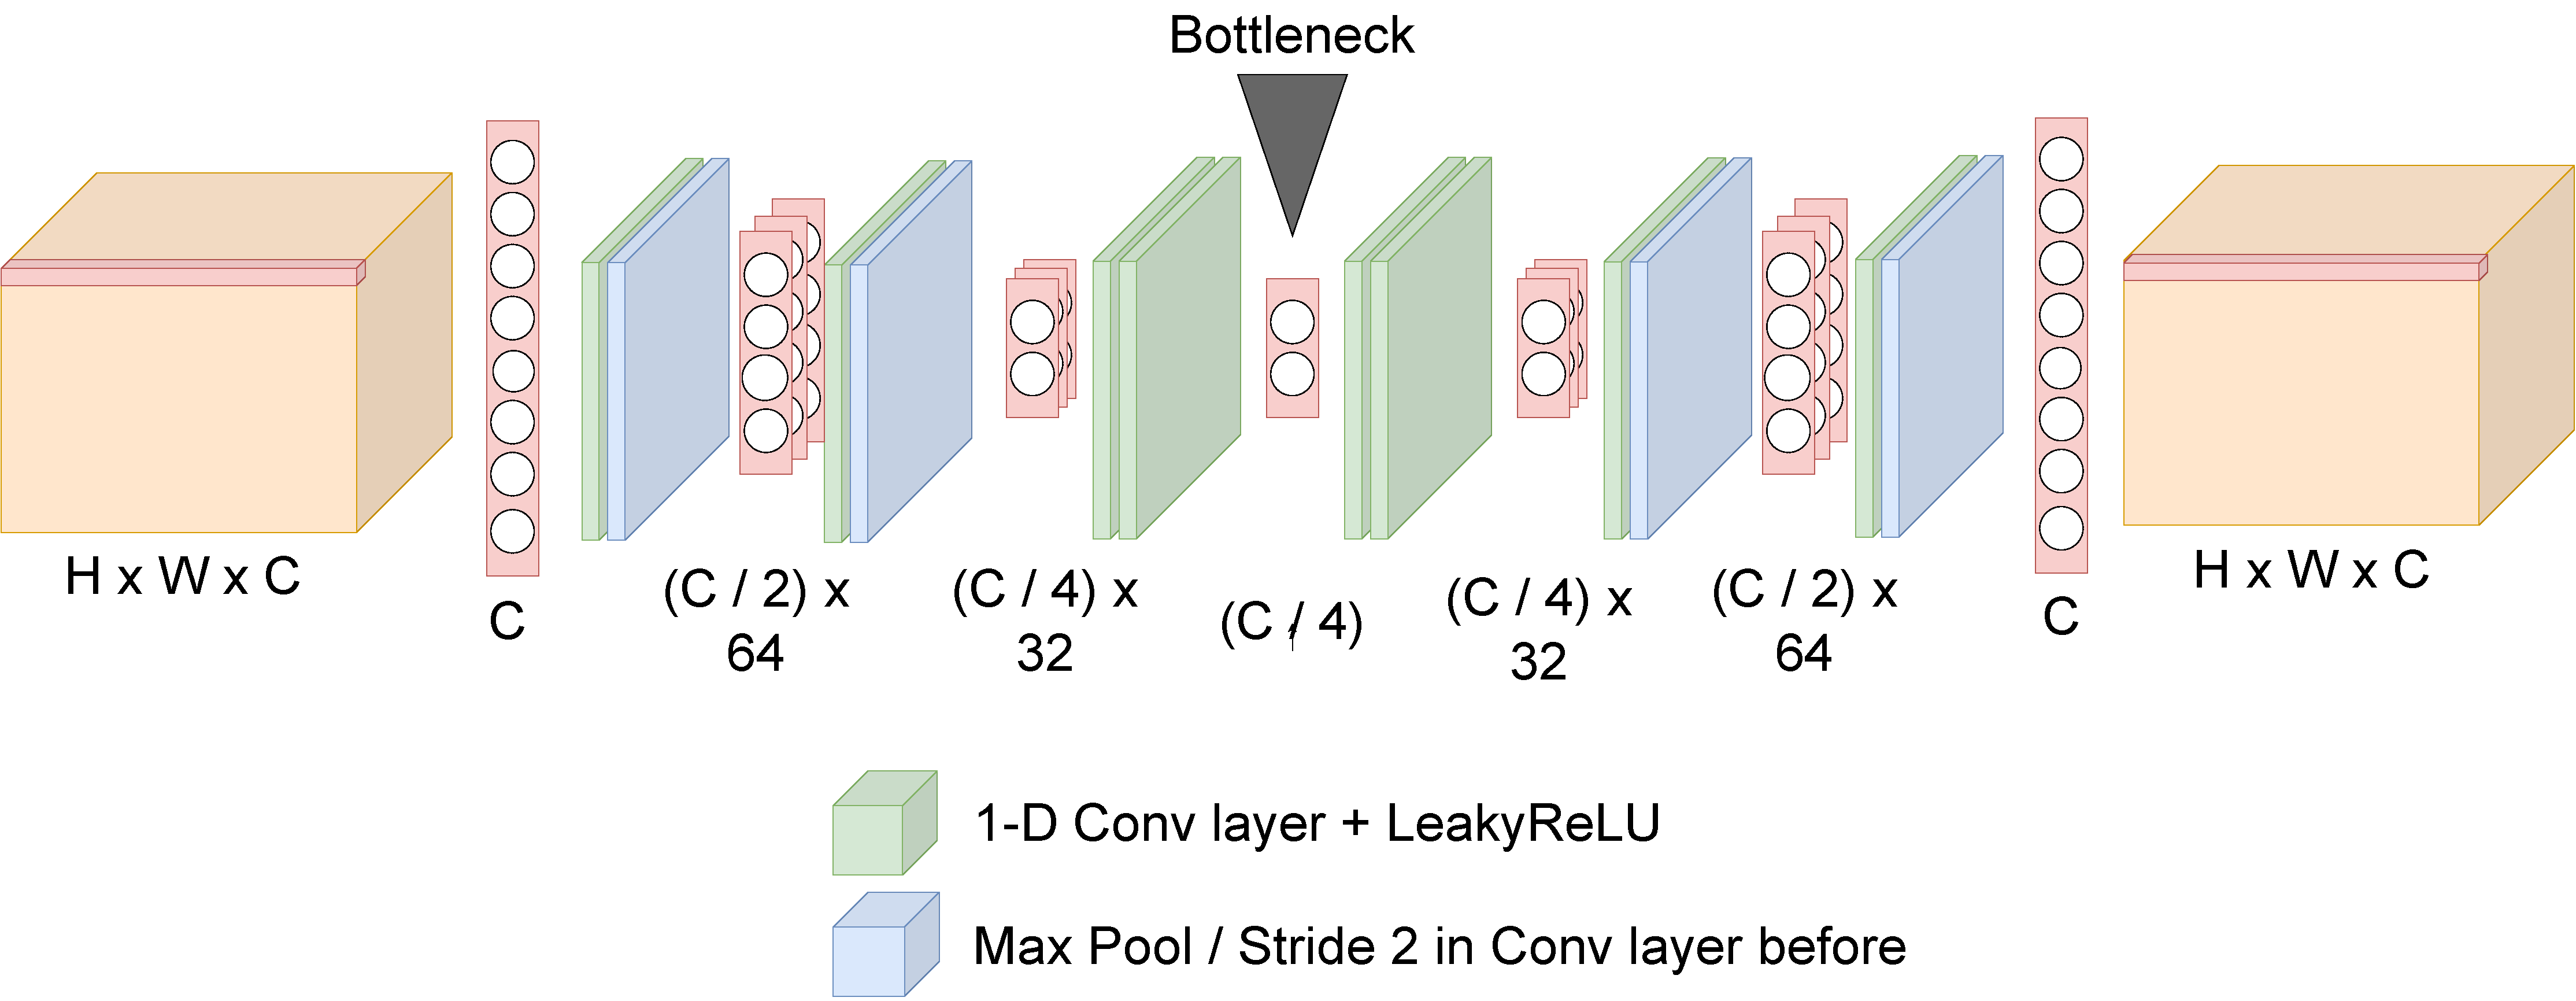
\includegraphics[scale=0.18]{img/OneDCNN.pdf}
\caption[Per-Pixel spectral \ac{cnn}]{Architecture of the per-pixel spectral \ac{cnn} using two downsampling layers resulting in a compression factor of four}
\label{fig:onedcnn}
\end{figure}
The first of the spectral autoencoder methods is based on the model proposed in Kuester et.al. \citep{kuester_1d-convolutional_2021,kuester_transferability_2022}. In their proposed method a hyperspectral input is split up into its pixels. The spectrum for each pixel then forms one datapoint on which the model is trained. The encoder of the model being trained is a \ac{oned} \ac{cnn} consisting of two sets of a \ac{oned} convolutional layer with a large kernel size of 11 and a max pooling layer followed by two additional \ac{oned} convolutional layers with a kernel size of 9 and 7. The number of filters is also reduced by a factor of two in each convolutional layer and set to one in the last layer, resulting in a bottleneck with one fourth of the original spectral channels. The decoder is built analogously, only replacing the max pooling layers by upsampling layers. After each convolutional layer a \ac{lrelu} is used as the activation function. Additionally, the number of channels are padded with channels containing zero values in order for them to be divisible by the downsampling factor of 2. Since the number of channels is reduced by a factor of twice the downsampling factor during encoding, this can result in the bottleneck not having exactly one fourth of the channels of the input, if the number of channels in the padded input is not divisible by four. The decoder then results in one channel more than the original input. In this case, the last channel of the output is removed. A whole image can be compressed by encoding and decoding each pixel of the image separately, then reassembling the output image from the decoded pixels. The architecture of this model is shown in \autoref{fig:onedcnn}.

This model is highly compatible with the combined model approach. Because the encoding of the spectral channels is performed per pixel, spatial dependencies are guaranteed to remain during encoding. The latent image is produced similarly to the output of the decoder by reassembling the latents for each pixel into a latent image, which can then be further encoded using a spatial autoencoder. In order to optimize the model for use in the combined model architecture and for the used dataset HySpecNet-11k \citep{fuchs_hyspecnet-11k_2023}, we adapted the model in various ways.

In the model as proposed by Kuester et.al. \citep{kuester_1d-convolutional_2021,kuester_transferability_2022}, the number of layers and therefore the compression ratio is fixed to four. However, different datasets can have different amounts of spatial and spectral dependencies. In the context of the combined model, this can result in the optimal model requiring a different spectral compression factor than 4. To allow for different compression ratio, the number of sets of a convolutional and a max pooling layer was made variable. In addition to this, the number of filters in each convolutional layer was adapted to the number of channels in the data. In the original paper, the first layer has a number of filters equal to half the number of padded channels of the data. We adapted the number of filters to the higher number of channels in the HySpecNet-11k dataset by keeping this ratio equal. This has the advantage that the number of filters is always appropriately divisible regardless of the number of layers ensured by the padding on the spectral channels of the input. We also changed the padding strategy. Instead of padding to a number of spectral channels divisible by half the compression ratio and then conditionally removing some number of channels at the output, we directly padded to a number of spectral channels divisible by the compression ratio. This removes the need for removing channels at the output, simplifying the model without loss of performance.

This spectral compression model is not only interesting for its applicability to the combined model. It is also the hyperspectral compression model with the highest reconstruction accuracy for multiple bitrates among many compared models. For more on this see \autoref{cha:chapter5}. However, there are also some disadvantages of the model architecture. The reduction of spectral channels using max pooling layers results in divisions by two in the number of channels. This means that the compression ratio can only be a power of two. Additionally, the higher the chosen compression ratio is, the higher the number of needed padding channels is. As an example, for the HySpecNet-11k dataset with 202 channels two padding channels are needed for the compression ratio 4, for a compression ratio of 32 14 padding channels would be needed. Finally, the training process of this model is much slower than for which take complete images as input. Since each pixel is compressed separately, the number of optimization steps per epoch is much higher. This is also further discussed in \autoref{cha:chapter5}.
\subsection{Two-dimensional Spectral CNN\label{sec:fastconv1d}}
To address the issues of the \ac{oned} spectral \ac{cnn}, we developed another model. This model uses \ac{twod} convolutional layers with a kernel size of one to compress a whole image at once. For convolutional layers with a kernel size of one the convolution operation collapses down to a scalar multiplication. Additionally, the output has the same height and width as the input, as each pixel in the output is calculated only from the channels of a corresponding input pixel. The output for a specific pixel and filter is therefore equivalent to a weighted sum over all channels in the input for this pixel. Importantly however, the weight used for a specific input channel is the same for each pixel in the image. A two-dimensional convolutional layer with a kernel size of one can therefore only encode spectral information when applied to a hyperspectral image, making it usable as part of the combined model. Such layers are commonly used for decreasing the number of filters between other convolutional layers TODO REF. Because of this, they are also referred to as channel or feature map pooling layers. They are then able to learn non-trivial summarizations of the preceding layer because of the nonlinearity introduced by the used activation function, in our case \ac{lrelu}. However, they can also instead be used to the opposite effect of increasing the number of filters while retaining the semantic information within these filters. An example of both of these uses is present in the "Inception" architecture proposed in Szegedy et.al. \citep{szegedy_going_2014}.

We show that it is also possible to use such layers to learn spectral dependencies in hyperspectral image data. The model is comprised of two-dimensional convolutional layers starting with a number of filters slighly higher than the number of channels in the hyperspectral dataset the model is trained on, 256. In each layer, the number of filters is doubled in order to increase the amount of information available. Finally, a last convolutional layer is used to reduce the number of channels to result in the desired bottleneck size. All convolutional layers use a kernel size of one and the \ac{lrelu} activation function.

This architecture has multiple advantages compared with the one-dimensional spectral \ac{cnn}. Instead of being applied per pixel, it can be applied to the entire image at the same time. It also requires less parameters, as each layer has a number of parameters equal to $N_p = C * F$, where $C$ is the number of channels of the input to the layer and $F$ is the number of filters in the layer. Both of these factors result in a much shorter training time as seen in \autoref{cha:chapter5}. The model is also more flexible with regard to the compression ratio. In contrast to the one-dimensional spectral encoder, where the compression ratios are necessarily given by $R \approx 2^N$, where $N$ is the number of pooling layers, the two-dimensional spectral encoder allows setting of the number of output channels to an arbitrary number. This also removes the need for padding, which is an advantage especially for high compression ratios which would otherwise require much padding. Furthermore, the one-dimensional spectral \ac{cnn} gets slower for higher compression ratios as it requires more layers while the number of layers and therefore the speed of the two-dimensional spectral \ac{cnn} is constant with respect to the compression ratio.

Two modifications were also tested for this model. First, a Layer Normalization was performed after each convolutional layer in order to improve generalization performance and further reduce training time.  We also modified the model by changing the kernel sizes of the convolutional layers. With higher kernel sizes, the model becomes able to incorporate some amount of local spatial dependencies in addition to the spectral dependencies. We used this to study how sensitive the combined model is to spatial dependencies being partially encoded in the spectral encoder/decoder.
\subsection{Variational autoencoder \label{sec:vae}}
As mentioned in \autoref{sec:combinedmodel}, a requirement for spectral encoder / decoder pair is that the decoder is able to decode the latent of the encoder after some distortion to it has been applied by the spatial autoencoder. Therefore, using a \ac{vae} for the spectral compression is interesting, because \acp{vae} produce a continuous latent space as shown by TODO REF. A \ac{vae} learns a probability distribution for a latent space and produces reconstructions by generating a samples from this distribution. We designed a one-dimensional \ac{vae} with the purpose of learning to autoencode spectral dependencies for single pixels, similar to the per-pixel \ac{cnn}. This per-pixel \ac{vae} in fact uses the per-pixel \ac{cnn} to produce a latent for a given input pixel. Two independent linear layers are then applied to this latent to produce a mean and a variance tensor respectively. The dimensionality of these vectors is variable and therefore a hyperparameter of the model. The linear layer producing the mean uses a tanh activation function to constrain the means between -1 and 1. The linear layer producing the variance also uses tanh but follows by an application of the softplus function to produce a positive variance. A new latent is then sampled from this distribution to produce the input for the decoder which is a symmetric inverted version of the encoder with only one linear layer instead of two, since only the new latent needs to be transformed to the latent space of the per-pixel \ac{cnn}.

A basic \ac{vae} has not yet been used for hyperspectral image compression. Especially compression of spectral signatures using a one-dimensional \ac{vae} has not been studied. The only \acp{vae} architecture commonly used for image compression is the hyperprior architecture, which is described in \autoref{cha:chapter4}. However, these models are not applicable to be a spectral autoencoder for the combined model for two reasons. First, hyperprior models so far have been used for spatial dependencies in images, being applied to whole images at once and not one-dimensionally to spectral signatures. Secondly, since hyperprior models use an arithmetic coder in the bottleneck, they can only be used as the last stage of a compression model since the output of the arithmetic coder cannot be further compressed using another model. This model attempts to overcome these limitations to produce a continuous latent space that can be further compressed using a spatial autoencoder method while being permissible with regard to distortions being introduced during this process.
\section{Spatial Autoencoder Methods\label{sec:spatialae}}
The second part of the combined model is the spatial autoencoder that further compresses the bottlneck of the spectral encoder. While there are some preconditions required for the spectral encoder/decoder pair, the choice of the spatial autoencoder is highly flexible. Since the latents of the spectral encoder have similar spatial dependencies to actual images, any autoencoder that is able to compress images can be used for this part of the model. The models analysed in this thesis are a \ac{cnn}-based autoencoder, a hyperprior model and an optimized hyperprior model using self-attention modules and a context model. We also analysed the use of \ac{jpeg} 2000 as the spatial autoencoder to study the viability of using a spatial autoencoder as part of the combined model that is not learning-based.
\subsection{CNN-based Spatial Autoencoder\label{sec:conv2d}}
The \ac{cnn}-based spatial autoencoder model uses a low-complexity approach using only two-dimensional convolutional layers. A similar architecture was used for hyperspectral image compression by La Grassa et.al. \citep{la_grassa_hyperspectral_2022}. However, there are multiple differences between the model. La Grassa et.al. use a linear layer as the final layer of their network. This was not done for the \ac{cnn}-based spatial autoencoder as it would increase the number of parameters of the model and therefore increase both training time and the required computational resources. The model proposed in this thesis also adds regularization into the model using layer normalization \citep{ba_layer_2016}. The number of filters in each layer is also different. Further, La Grassa et.al. uses max pooling layers to reduce the spatial dimensionality of the latent while we use convolutional layers with a stride. Additionally, we experiment with different kernel sizes to vary the amount of spatial dependencies introduced to the autoencoder.

The \ac{cnn}-based spatial autoencoder model first uses two-dimensional convolutional layers to increase the dimensionality of an input image. This is done by using number of filters much higher than the number of channels in the input. This input layer is followed by another convolutional layer with the same number of filters to increase the depth of the model. Following that is a convolutional layer with a stride of two to reduce the spatial dimensions. This layer also increases the number of filters in order to reduce the information loss while downsampling. Finally, two further convolutional layers reduce the filter dimension to be identical to the number of channels in the input. In this way the dimensionality of the input is reduced by a factor of two in each spatial dimension, resulting in an overall compression factor of four. Additional layers with a stride of two can be added to increase the compression factor. The decoder is symmetrical to the encoder but replaces convolutional layers with transposed convolutional layers. The model uses the \ac{prelu} activation function after each convolutional layer and the sigmoid activation function after the final layer of the encoder and the decoder to keep outputs in the interval $[0,1]$. Layer normalization \citep{ba_layer_2016} is also performed after each convolutional layer to increase robustness and rate of convergence during training. Layer normalization was used instead of the more common batch normalization because it is able to perform well even with a low batch size and the combined model with the per-pixel \ac{cnn} was trained using a batch size of one.

This model was deliberately designed to be low-complexity to reduce the confounding factors for studying properties of the combined model. As there is no prior research for combining models in the way it was performed in this thesis for hyperspectral or \ac{rgb} image compression, the properties of the combined architecture as a whole was a focus of the experiments. A low-complexity spatial model is therefore a useful baseline that allows for better attribution of specific experimental results to the combined architecture.
\subsection{Hyperprior-based Spatial Autoencoder}
To also include a more complex model with high relevancy in \ac{rgb} compression research, we implemented the scale hyperprior model proposed by Ballé et.al. \citep{balle_end--end_2017}. Since this model was explored in detail in \autoref{cha:chapter4}, we will not go into detail here. The only necessary adaptation to the model in order to use it as part of the combined model was a change of the input and output layer to accomodate the chosen number of channels in the latent of the spectral encoder. This model was not studied intensively but rather used as a baseline. The main hyperprior-based architecture used was the following model using self-attention modules and a context model.
\subsection{Attention-based Model Using Hyperprior Architecture\label{sec:atthyperprior}}
The main hyperprior-based model that was studied is based on work by Cheng et.al. \citep{cheng_learned_2020}. They further improve the joint autoregressive and hierarchical hyperprior model by Minnen et.al. \citep{minnen_joint_2018} discussed in detail in \autoref{cha:chapter4} by introducing self-attention modules. The attention modules are based on work by Liu et.al. \citep{liu_non-local_2019}. However, the non-local blocks have been removed in order to simplify the attention modules. This allowed them to reduce the complexity of the model while still being able to adequately capture long-range dependencies in the data. These self-attention modules were inserted into the main encoder and decoder in two places as shown in Fig. TODO.

We adapted this model in multiple ways for use in the combined model. First, the model was adapted to be able to receive different numbers of input channels by changing the input and output layers. The second modification regards the strength of the spatial downsampling in the convolutional parts of the hyperprior model. In the original model the main encoder reduces the spatial dimensionality by a factor of 8 in each direction, 64 in total, to produce the latent that is input to both the arithmetic coder and the hyperprior encoder. The hyperprior encoder reduces the spatial dimensions by a factor of 4 in each direction, 16  total, again. Since they used a dataset with 256x256 pixels, this results in a bottleneck of size 32x32 after the main encoder and 8x8 after the hyperprior encoder. However, for hyperspectral data in general and the HySpecNet-11k dataset especially a reduction in spatial dimension with a factor of 64 can result in large distortion, since there are less spatial dependencies than in typical \ac{rgb} datasets. We therefore modified both the numbers of convolutional layers and the strides in the main encoder/decoder pair and the hyperprior encoder/decoder pair in order to allow for different options for the spatial dimensionality reduction factors. For this, we group models by the spatial reduction factors in the main encoder/decoder pair and the bottleneck size of the hyperprior encoder. The bottleneck size of the hyperprior being larger results in more information remaining present in the hyperprior which increases performance. However, more side information needs to be transmitted, which can decrease performance. This is because the loss used for training these models, \ac{rd} loss, tries to achieve a balance between bitrate and distortion. Since a larger amount of transmitted side information raises bitrate, \ac{rd} loss with the same parameters will also result in higher distortion. Therefore, an optimum needs to be found depending on the amount of spatial dependencies present in the dataset.
    \thispagestyle{fancy}
    \acbarrier
    \chapter{Experiments\label{cha:chapter5}}
This chapter describes the implementation of component X.

\section{Description of the Data Set\label{sec:xx}}

\section{Design of Experiments\label{sec:yy}}

\section{Loss Functions and Metrics}

\subsection{MSE Loss}

\subsection{Rate Distortion Loss}

\subsection{Dual MSE Loss}

\subsection{Metrics}

\section{Results of the XX\label{sec:ch5xx}}

\section{Results of the YY\label{sec:ch5yy}}

\section{Results of the ZZ\label{sec:ch5zz}}
    \thispagestyle{fancy}
    \acbarrier
    \chapter{Conclusion and Discussion\label{cha:chapter6}}

    \thispagestyle{fancy}

% ---------------------------------------------------------------
\backmatter % no page numbering from here
    
		
		% if you want to provide a glossary with explanations of important terms put it in here

    %\bibliographystyle{unsrt}
    %\bibliography{./bib/references}
    %
    \printbibliography

    \addchap{Appendix A}
	
\appendix
\begin{figure}
    \centering
	\pgfplotstableread[col sep=semicolon,]{graphs/freezedualmse.csv}\datatable
	\begin{tikzpicture}
	\begin{axis}[
		grid=both,
	    height=7cm,
	    width=\textwidth,
	    legend style={at={(0.95,0.45)},anchor=south east},
	    xtick={0,0.1,...,1},
	    ylabel={Spectral angle (degrees)},
	    xlabel={Dual MSE $\lambda$}]
	    
	    \addplot table [x={lmbda}, y={sangle_test}, 
	    restrict expr to domain={\thisrow{model_id}}{1:1}]{\datatable};
	    \addlegendentry{Combined-AllFrozen}
	    
	    \addplot table [x={lmbda}, y={sangle_test}, 
	    restrict expr to domain={\thisrow{model_id}}{2:2}]{\datatable};
	    \addlegendentry{Combined-EncoderFrozen}
	    
	    \addplot table [x={lmbda}, y={sangle_test}, 
	    restrict expr to domain={\thisrow{model_id}}{3:3}]{\datatable};
	    \addlegendentry{FastCombined-AllFrozen}
	    
	    \addplot table [x={lmbda}, y={sangle_test}, 
	    restrict expr to domain={\thisrow{model_id}}{4:4}]{\datatable};
	    \addlegendentry{FastCombined-EncoderFrozen}
	    
	    \addplot table [x={lmbda}, y={sangle_test}, 
	    restrict expr to domain={\thisrow{model_id}}{5:5}]{\datatable};
	    \addlegendentry{FastCombined-NothingFrozen}
	\end{axis}
	\end{tikzpicture}
	\caption{Dual MSE lambda plot}
	\label{fig:dualmselossangle}
	\end{figure}
	
\begin{figure}
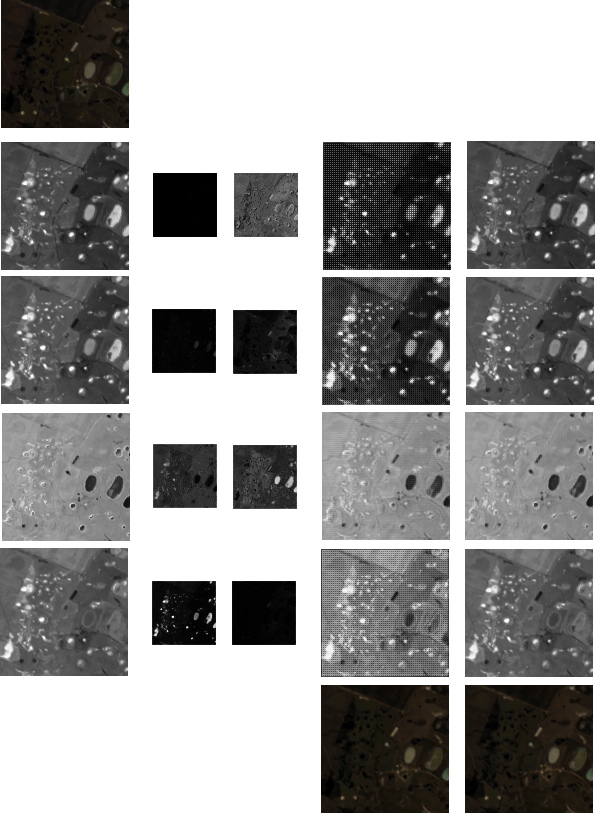
\includegraphics[scale=0.5]{img/latents_2.png}
\caption{Latent image comparison}
\label{fig:latentcompare2}
\end{figure}
\endinput


\end{document}
